\documentclass[11pt]{article}
\newcommand\tab[1][1cm]{\hspace*{#1}}
\newcommand\back[1][-3cm]{\hspace*{#1}}
\usepackage{graphicx}
\usepackage{soul}
\graphicspath{ {./eprog/} }
\begin{document}
\title{introduction to programming}
\section{objects and classes}
\subsection{object}
Is a software machine that allows other elements to access (query) and modify (command) a collection of data. F.e an object can represent a city or a button.
\\\\Each object belongs to a class that defines the features or operations one can call on this class. It allows other software to access data on modify data on this object (read/write).
\\ An object is an instance of a class.
\\ Objects only exist during the runtime of a program.
\subsubsection{object oriented programming}
In object oriented programming you model objects of the real world into physical/abstract or software object.
\subsection{class}
A class is a sort of category for an object. All objects of a class share the same properties (a class is like a category of things, type).
\\ A program is a model.
\\ A class is the generating class of an object.
\\ Classes only exist in the software text.
\subsection{architecture}
Architecture is the design of a program into it's classes and the relations between them.
\subsection{implementation}
Writing the instructions (algorithms) and data structures of the classes.
\section{interfaces and information hiding}
\subsection{clients and suppliers}
A client of a software mechanism is any sort of system that uses it. f.e person or other software(electronic system).
\\ The software mechanism is the supplier to the system. f.e. class or group of classes.
\\ Arrow always goes from client to suppliers.
\subsection{interface}
An interface is the description of the techniques enabling clients to use it.\\
A program interface is an interface where the client is other software. API: Abstract Program Interface. 
\subsection{API's}
Objects are characterised by the operations clients may apply on them.
\paragraph{queries}
Operations that return the state or information of an object.
\paragraph{commands}
Operations that change the state of an object.
\\\\ The interface is how we (the client) are going to see the object.
Most of the time we do not wan't to see the implementation behind an object and we only wan't to see the interface = Information hiding.
\paragraph{information hiding}
The designer of the class must decide which properties are accessible to the clients and which are internal(only for the purposes of the class itself (public and secret)).
\section{Commands and queries, uniform access principal}
\subsection{Features: commands and queries}
Every feature call, will always be called on a object (your\_object.your\_feature). A feature is an operation available on a certain class of objects. Their are three kinds of features:
	\\Commands\\Queries\\Creation procedures
	\paragraph{Queries} calling a query should not change the answer the program gives back! The goal of a query is to obtain information about the object without modifying it.
	\paragraph{Commands} change the properties of one or multiple objects.
\subsection{Routines, procedures, functions, attributes, and the Uniform Access Principle}
\subsubsection{Routine (=method )}
Removing details specifics and capturing the essence of the information.\\ In programming there are two sorts of abstractions: \\Data abstraction, done with a class.\\Computational abstraction (algorithms) done with routines.\\Example of a routine in Eiffel:\\r(arg: type)\\require\\\tab preconditions...\\do\\\tab instructions...\\ensure\\\tab  postconditions...\\end
\subsubsection{Uses of routines}There are two different uses for Routines:\paragraph{bottom-up:} Encapsulating a computation for reuse.\paragraph{Top-down:} Calling a routine before having written it. Allows to write the bigger code at the beginning and go to the little details later.
\subsubsection{Kinds of routines}
Their are two kinds of routines:\paragraph{Procedure:} doesn't return a result.\paragraph{Function:} returns a result(f(arg: type):result type).\\
\back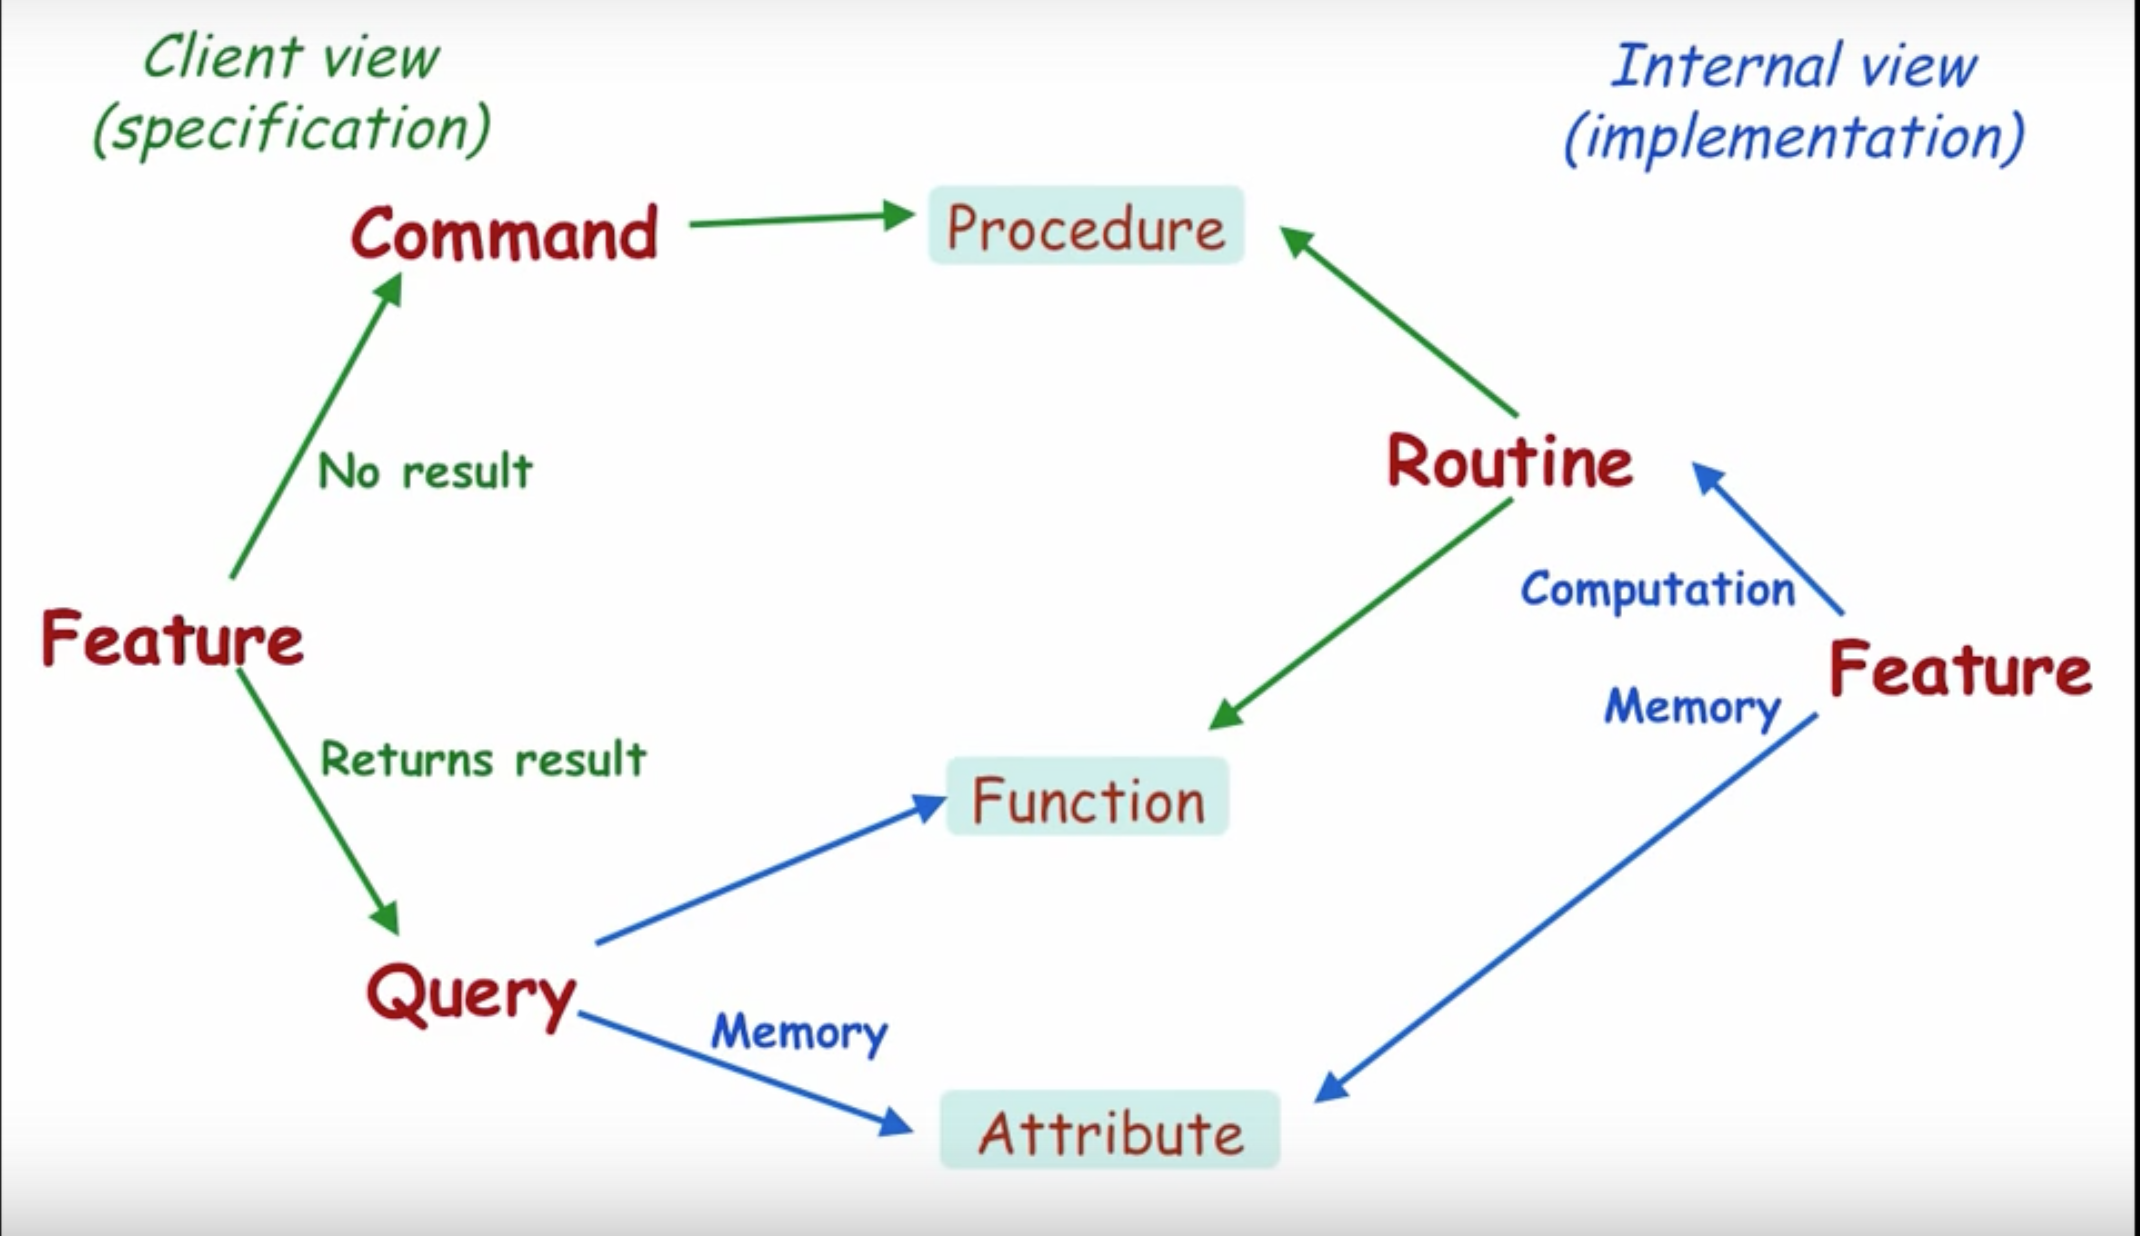
\includegraphics[scale = 0.5]{feature}
\subsubsection{Attributes}
Each class has an attribute field where there is every object of this class in the program.
\subsubsection{The uniform access principal}
Features should be accessible to the client in the same way wether implemented by storage or by computation(it does not matter if what you are looking for already exists in the memory or if you have to compute it from some other pieces of memory(in the image function and attribute are therefore equal)). 
\section{Object creation}
\subsection{basics}
\subsubsection{Identifier}
An identifier is a name chosen to describe certain elements of the program such a class, feature or object.\\ An identifier that denotes a value at runtime is called an \hl{entity}.\\ If the value of an entity can change during runtime it is called a \hl{variable}.\\ An entity detonating an object is \hl{attached} to this object. 
\subsubsection{Object creation}
First you create an object in memory and then attach an entity to it. First you have to declare the entity with a certain type (leg1: LEG). Then you create leg1(create leg1). Leg1 will then be created during runtime and initialised with the default values.\\ If you want to create an object with other than the default values, you can create \hl{creation procedures} for the class.\\\\class point create\\\tab default\_create, make\_cartesian, make\_polar\\feature\\\tab...\\end\\\\ You then have to declare these creation procedures in the feature. Then you can declare the object as(create point.make\_polar(r,t)) (create point == create point.default\_create).
\subsection{Void references}
\subsubsection{Initial state of an object}
Initially, before the creation of an object, it's reference is void. During execution a reference is either \hl{void} or \hl{attached}(to find out you can write x=void or x/=void).
\subsubsection{Utility of void references}
For example in a linked list, to know where the list ends the next next reference of the last element of the list is void.\\ Void references do cause trouble however \hl{(you cannot call a feature on a reference wich is void)}. Eiffel is void safe, therefore the code will not compile if the code might cause a void call.

















\end{document}
